\documentclass[letterpaper,12pt]{article}
\usepackage{tabularx} % extra features for tabular environment
\usepackage{amsmath}  % improve math presentation
\usepackage{graphicx} % takes care of graphic including machinery
\usepackage[margin=1in,letterpaper]{geometry} % decreases margins
\usepackage{cite} % takes care of citations
\usepackage[final]{hyperref} % adds hyper links inside the generated pdf file
\hypersetup{
	colorlinks=true,       % false: boxed links; true: colored links
	linkcolor=blue,        % color of internal links
	citecolor=blue,        % color of links to bibliography
	filecolor=magenta,     % color of file links
	urlcolor=blue         
}
\usepackage{blindtext}
%++++++++++++++++++++++++++++++++++++++++


\begin{document}

\title{\textbf{A monitoring network of static electric field and lightning at the Pierre Auger Observatory}}
\author{J. Peña-Rodríguez and L. A. Núñez$^1$ \\
P. Salgado-Meza and L. Flórez-Villegas$^2$}


\date{$^1$\small Escuela de Física, Universidad Industrial de Santander\\%
    $^2$Escuela de Ingeniería Electrónica, Universidad Industrial de Santander\\[2ex]%
\today}
\maketitle

\begin{abstract}
In this work, we expose the preliminary results of the implementation of a weather station for monitoring the atmospheric electric field and lightning during thunderstorm episodes for studying its effect on the secondary particle flux at ground level at the Pierre Auger Observatory. The atmospheric electric field during thunderstorms can increase above hundreds of kV/m causing an acceleration in charged particles composing secondary cosmic rays. Such acceleration causes avalanche processes in the atmosphere enhancing or reducing the particle flux at ground level depending on the strength and polarity of the electric field.
\end{abstract}

\section{Introduction}

Cosmic rays (CRs) are particles reaching the Earth after crossing interstellar space. High energy CRs originate outside the solar system and most of the low-energy ($<$ 10 GeV) particles have a solar origin. When CRs enter the terrestrial atmosphere, they interact with the atoms generating Extensive Air Showers (EAS) of secondary particles \cite{Spurio2015}.

Secondary particles, mainly electrons/positrons, can be affected by the atmospheric electric field. They can be accelerated \cite{marshall2005observed} causing Relativistic Runaway Electron Avalanches (RREA) \cite{dwyer2011low} increasing the secondary flux at ground level. The atmospheric electric field can rise up to hundreds of 100 kV/m during thunderstorm episodes. The minimum electric field for triggering an RREA is roughly 286 kV/m \cite{Skeltved2017, colalillo2019}. Some investigations demonstrate the flux of heavier particles such muons can also be modulated by the atmospheric electric field \cite{wang2012effect, alexeenko2002transient}.

The flux variation of charged particles depends on the polarity of the atmospheric electric field \cite{bartoli2018observation, zhao2019effects}. During negative electric fields, negative charge particles are accelerated towards the ground enhancing the particle counting at the detector level. On the other hand, in the presence of a positive electric field, the counting ratio at ground level decreases \cite{dorman2013cosmic}. These observations give an explanation of the electron/positron flux variation which has been observed by CRs observatories during thunderstorms.

The lack of electric field monitoring networks inside CR observatories limits the understanding of the underlying phenomena responsible for the recorded anomalous events \cite{Colalillo2017, Merenda2019}. The data cross-checking between the particle counting rate and the transitory electric field shall help to clarify such phenomena.

We present the preliminary results of the development of a modular monitoring station capable to measure slow ($<$ 100 Hz) and fast ($<$ 500 KHz) changes in the atmospheric electric field during thunderstorm episodes. The station allows us to create a temporally synchronized network for finding correlations between secondary flux and electric field variations, as well as, it is able to estimate the localization of lightning strike points.

\section{Quasi-static electric field}

Slow variations (0.1\,Hz to 1\,kHz) of the atmospheric electric field are caused by the charge accumulation inside the clouds. Such variation is initially generated by charge drift and diffusion \cite{gunn1957experimental}. Another mechanisms take part during the cloud development: ionic selection (ionic capture by polarized drops) \cite{stow1969atmospheric} and the rupture of large water drops\cite{matthews1964electrification}. When the cloud is totally formed, the electric charge variation is dominated by inductive, convective, thermoelectric, and interface mechanisms \cite{vonnegut1955possible, latham1961generation}.

There exist several technologies for measuring slow variations of the atmospheric electric field. These are inductive probes, field mills, and optical sensors \cite{miles2009report}. E-field mills are widely used to measure slowly-varying electric fields associated with cloud charging processes. 

\begin{figure}[h]
\begin{center}
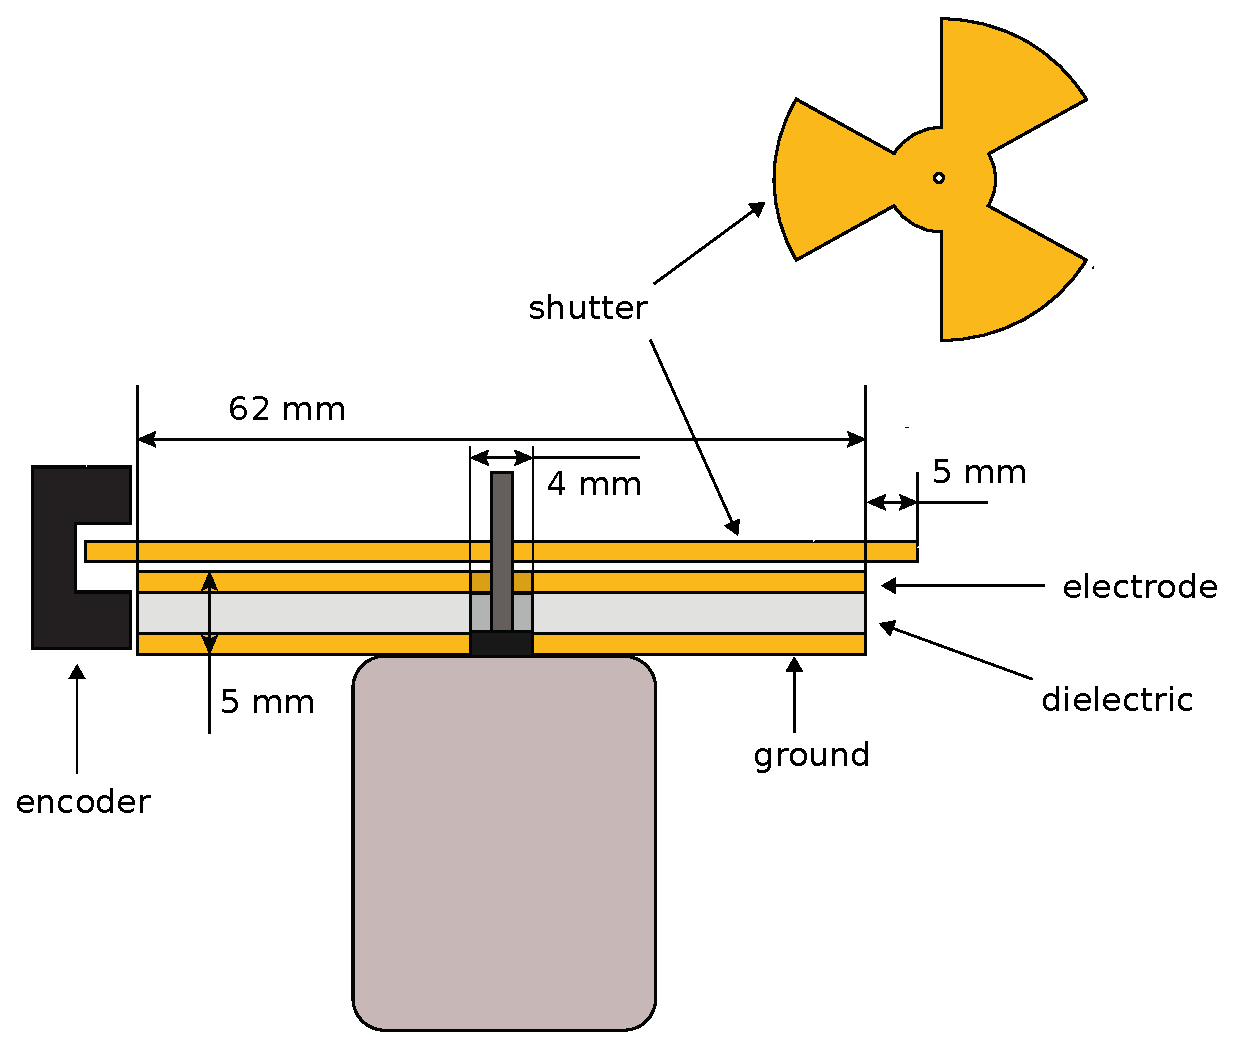
\includegraphics[width=.45\textwidth]{Figures/Emill.eps}
\caption{\label{emill} Mechanical structure of the E-field mill. The shutter is made by a three-blade copper plate 72 mm diameter which covers a 62 mm diameter sensing electrode. A 6\,pF capacitor is formed between the sensing electrode and the ground plate with a 2\,mm acrylic layer as the dielectric material. The encoder is placed on the side of the capacitor.}
\end{center}
\end{figure}

In the E-field mill, the steady electric field is shielded and unshielded by a moving grounded shutter placed over a sensing electrode. The charge induced on the sensitive electrode flows to the ground when the shutter screens the external electric field and flows back to the sensing electrode when it is uncovered. The resulting sinusoidal current is proportional to the electric field magnitude \cite{Rakov2016}.  

The implemented E-field sensor is composed of three Bakelite plates (shutter, sensing electrode, and ground). Each plate 1.4\,mm width with a copper layer of 35\,$\mu$m. The dielectric was made of a 2\,mm acrylic layer. The sensing electrode has a diameter of 62\,mm and three blades separated by 120$^{\circ}$. The shutter radius is 5\,mm larger than the sensing plate in order to interrupt the encoder for generating the signal phase. The ground plate is connected to the DC motor chassis. The estimated E-field mill capacitance is around 6\,pF. A complete sketch of the E-field mill structure is shown in Fig. \ref{emill}.

In order to improve the sensor sensitivity, we performed an evaluation of the induced voltage on the sensing plate and the rotation frequency of the DC motor which is a third of the frequency of the generated signal due to the sensing plate shape. The signal frequency spanned from 200 to 600\,Hz observing output voltages from 8 to 14\,Vpp. Taking into account the power consumption, vibrations and auditory noise we selected a signal frequency of 260 Hz which means a motor rotation frequency of 87\,Hz. 

\subsection{Signal conditioning}

The sensor prototype front-end is composed of a resistive measuring range selector, an op-amp follower for impedance coupling, an input DC decoupler, and an op-amp adder for the signal baseline setting as shown Fig. \ref{emill_c}. 

\begin{figure}[h]
\begin{center}
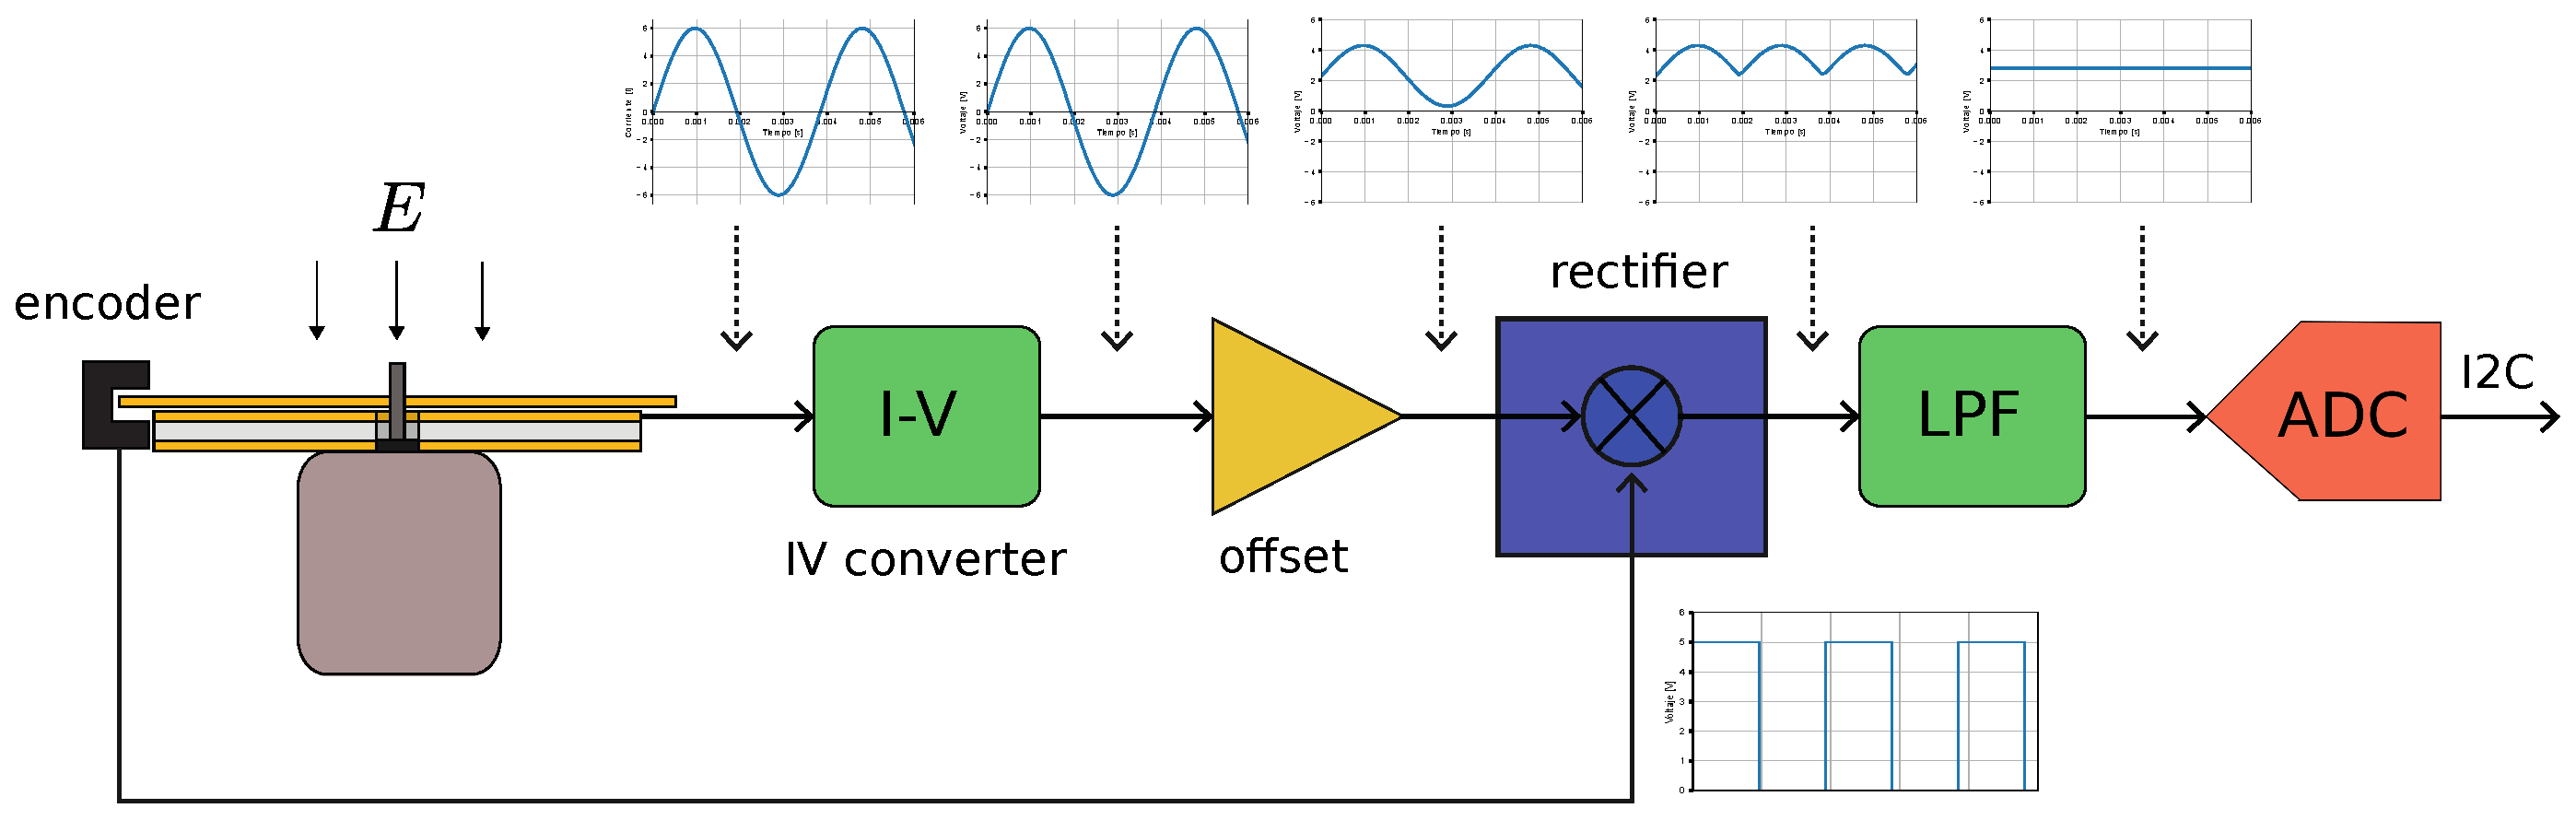
\includegraphics[width=1\textwidth]{Figures/Emill_esquema.eps}
\caption{General schema of the signal conditioning hardware. The current provided by the sensitive plate under the influence of an external electric field is converted to a voltage signal by means of an IV converter. An adder fixes the signal baseline in the middle of the precision rectifier input range ($\sim$2.25\,V). The rectifier output is smoothed by a low pass filter (LPF) before the digitization.}
\label{emill_c}
\end{center}
\end{figure}

The sensor measuring ranges are selected by jumpers JP1 (0-200\,kV/m), JP2 (0-60\,kV/m), and JP3 (0-500\,kV/m). The output sinusoidal signal varies from 0 to 5 V around a baseline of 2.25 V.

One of the advantages of mill sensors, is they determine the induced field direction by means of comparing the rotation phase of the shutter and the phase of the sensing plate signal using a precision rectifier. For carrying out such operation, we used the Mixer component of the Programmable System on Chip (PSoC 5LP from Cypress Semiconductor). The rectification task requires as input the E-field mill signal, the phase digital signal generated by an encoder (EE-SJ3), and the reference voltage which indicates the DC level over which the comparison occurs.

The Mixer inverts the sinusoidal signal when the phase is 0. The resulting modulated signal has a RMS value proportional to the magnitude of the induced electric field. The signal ripple is smoothed by a low-pass filter. We used a 1000 $u$F capacitor connected in parallel to the output with a frequency cut of $\sim$ 0.2\,Hz.

\subsection{Signal digitization and signal transmission}

The signal digitalization is performed by a 20-bit delta-sigma ADC. The ADC is integrated in the PSoC 5LP with a single-ended configuration, a sampling frequency of 183\,SPS (Samples Per Second), and an input range from 0 to 5\,V. One ADC unit is equivalent to 4.5\,$\mu$V.

The digitized E-field data is transmitted by I$^{2}$C protocol with a speed of 100\,kbps. The I$^{2}$C module was controlled by a $C$ script. The code configures the sensor initialization, device address (0x60) and memory sub-addresses. Since the communication protocol sends 8-bit data packages, the ADC data (20 bits) is split into 4 8-bit-blocks stored in the device sub-addresses from 0x00 to 0x03.

\subsection{Calibration}

\begin{figure}[h]
\begin{center}
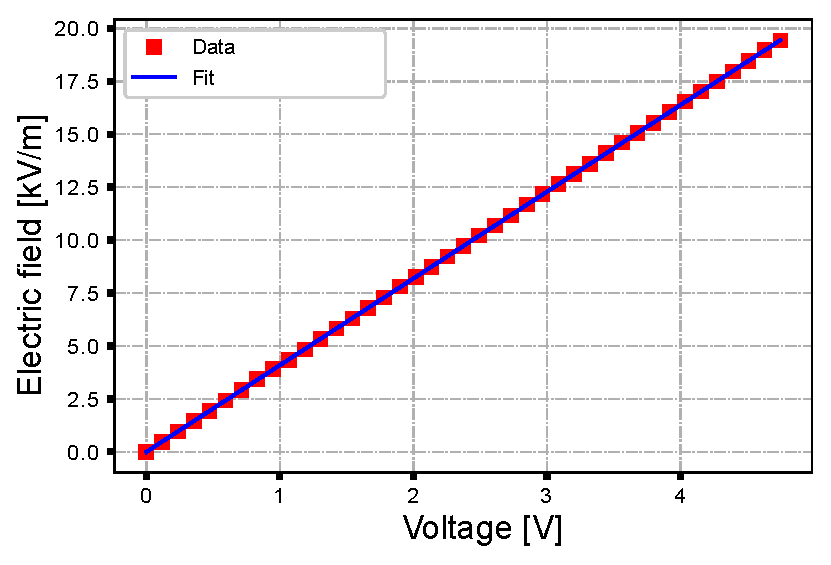
\includegraphics[width=0.48\textwidth]{Figures/Fuente_E.eps}
\includegraphics[width=.5\textwidth]{Figures/emill_v2.pdf}
\caption{\label{cal_fuente} Characterization curve of the E-field generator depending on the control voltage (left). Calibration curve of the E-field mill as a function of the induced electric field from 0 to 20 kV/m (right).}
\label{cal_fuente}
\end{center}
\end{figure}

The E-field sensor calibration was performed using a controlled E-field generator following the methodology proposed by Cui et. al. \cite{cui2017}. The field generator was a squared capacitor made of two parallel plates 20 cm side and 10 cm separation. A DC/DC EMCO C20 power source provided the high voltage applied between the generator plates. The generator was controlled by a Raspberry Pi board by means of a 12 bits DAC MCP4725 generating a E-field range of 0-20\,kV/m with a resolution $\sim$5\,V/m. The characterization curve of the E-field generator is displayed in Fig. \ref{cal_fuente}-left. The sensor was located inside the parallel capacitor under E-fields ranging from 0 to 2\,kV/m with $\sim$400\,V/m steps. The sensor calibration curve is shown in Fig. \ref{cal_fuente}-right.

\section{Lightning}

Charge accumulation inside thunderstorm clouds can break down the resistance of air unchaining fast variations (1\,kHz-1\,MHz) of the atmospheric electric field: the most common is lightning. Peculiar events recorded by cosmic ray observatories as the Pierre Auger match with such fast variations. We propose a lightning monitoring network to understand the phenomena underlying such events. 

\subsection{Detection hardware}

A parallel plate antenna composes the lightning detection system front-end. The device detects the E-field variation during lightning discharges. An active integrator converts the antenna current in a voltage proportional to the induced E-field. A fast ADC digitizes the voltage signal, and a NOR Flash memory temporally stores it. A voltage-over-threshold trigger system determines the event truthfulness starting the information transmission towards the single computer board (Raspberry Pi 2). Fig. \ref{diagrma_cam_rap}  shows a diagram of the detection system.

\begin{figure}[h!]
\begin{center}
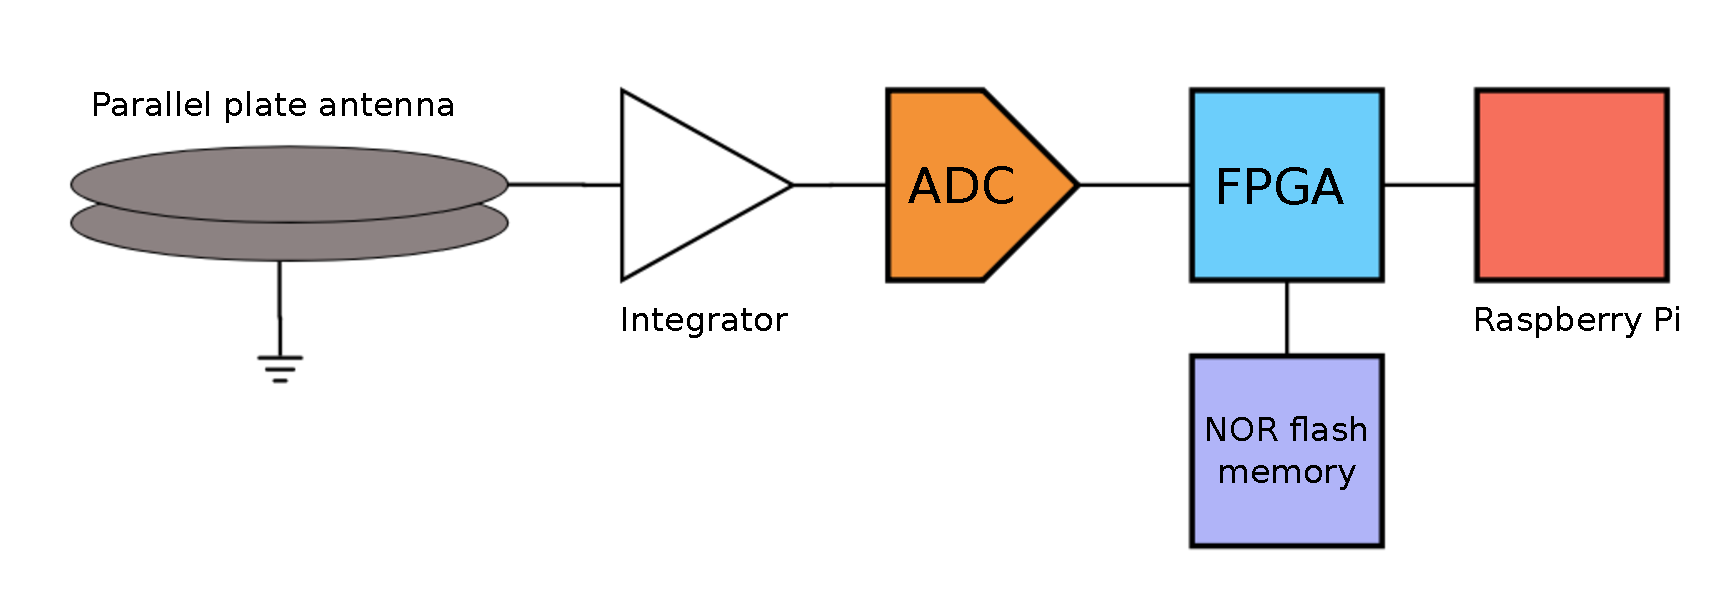
\includegraphics[width=0.9\textwidth]{Figures/Fast.eps}
\caption{Lightning data acquisition system. A parallel-plate antenna detects the lightning signal; an active integrator converts the signal in a voltage proportional to the induced electric field. A fast ADC digitizes the signal, and a voltage-over-threshold trigger, implemented on an FPGA, validates the event temporally stored in a NOR flash memory.}
\label{diagrma_cam_rap}
\end{center}
\end{figure}

\subsection{Antenna}

The parallel-plate antenna consists of two circular aluminum plates 40\,cm diameter separated by 2\,cm \cite{salgado2020}. The top plate senses the electric field, while the lower one is grounded. The antenna transmits the signal using an RG51 coaxial cable with a BNC connector end. Fig. \ref{antena_rap} displays the antenna structure.

\begin{figure}[h!]
\begin{center}
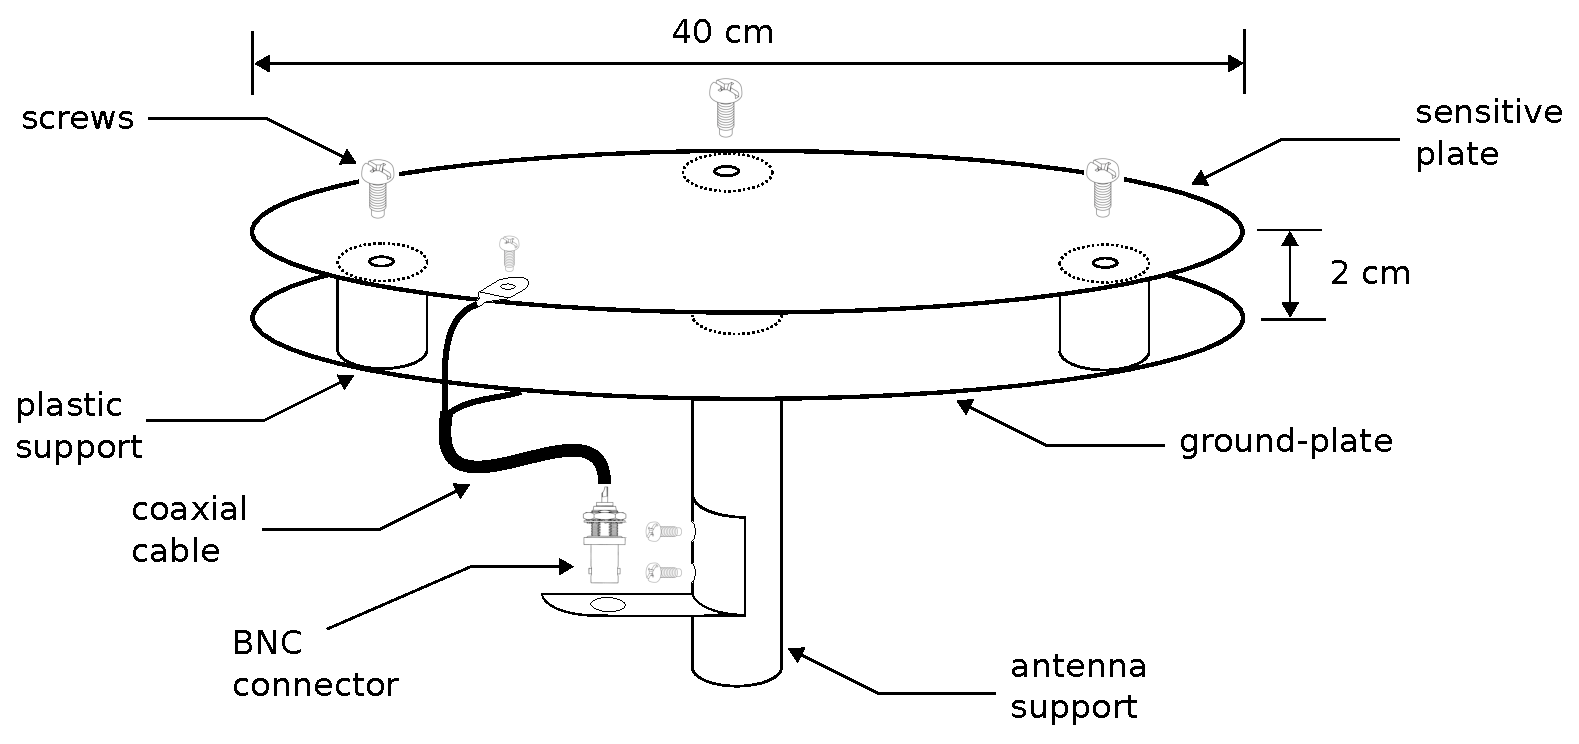
\includegraphics[width=0.8\textwidth]{Figures/Parallel_plate.eps}
\caption{Structure of the parallel-plate antenna. Two aluminum plates 40\,cm diameter separated by 2\,cm constitute the lightning sensor. A coaxial cable connected to a BNC transmits the antenna signal. The bottom plate is grounded.}
\label{antena_rap}
\end{center}
\end{figure}

The antenna current due to the induced electric field $E$ is

\begin{equation}\label{equ_inte}
I=\epsilon A \dfrac{dE}{dt}
\label{eq::antennacurr}
\end{equation}
\noindent where $A$ is the aluminum plate area and $\epsilon$ is the dielectric material permittivity. 

\subsection{Integrator}

We can deduce from Eq. \ref{eq::antennacurr} that the integration of the antenna signal gives us an estimation of the induced electric field as follows,

\begin{equation}\label{equ_inte}
V = \frac{1}{C} \int I dt = \frac{\epsilon A E}{C}
\label{eq::antennavol}
\end{equation}
\noindent where $C$ is the antenna capacitance. The measured electric field is

\begin{equation}\label{equ_inte}
E = \frac{CV}{\epsilon A}
\label{eq::antennaE}
\end{equation}
We implemented an active integrator on an OPA4228 operational amplifier. The op-amp has a 120\,dB CMRR and a bandwidth of 33\,MHz. An adder cascades the integrator to invert the signal and increase the baseline. Fig. \ref{fig::integrator} shows the circuit.

\begin{figure}[h!]
\begin{center}
\includegraphics[width=0.8\textwidth]{Figures/Integrador_circuito.png}
\caption{Front-end electronics circuit. The integrator (red-square) converts the antenna current in a voltage signal proportional to the induced electric field. An adder (blue-square) increments the baseline.}
\label{fig::integrator}
\end{center}
\end{figure}

The circuit frequency cut was estimated $\sim$10.6\,MHz. The frequency response of the circuit was simulated en PSpice and tested by varying the input frequency from 100\,Hz to 20\,MHz \cite{salgado2020}. The Bode diagram of the integration stage is shown in Fig \ref{fig::bode}. The measured frequency cut was located at $\sim$4\,MHz (-3\,dB).

\begin{figure}[h!]
\begin{center}
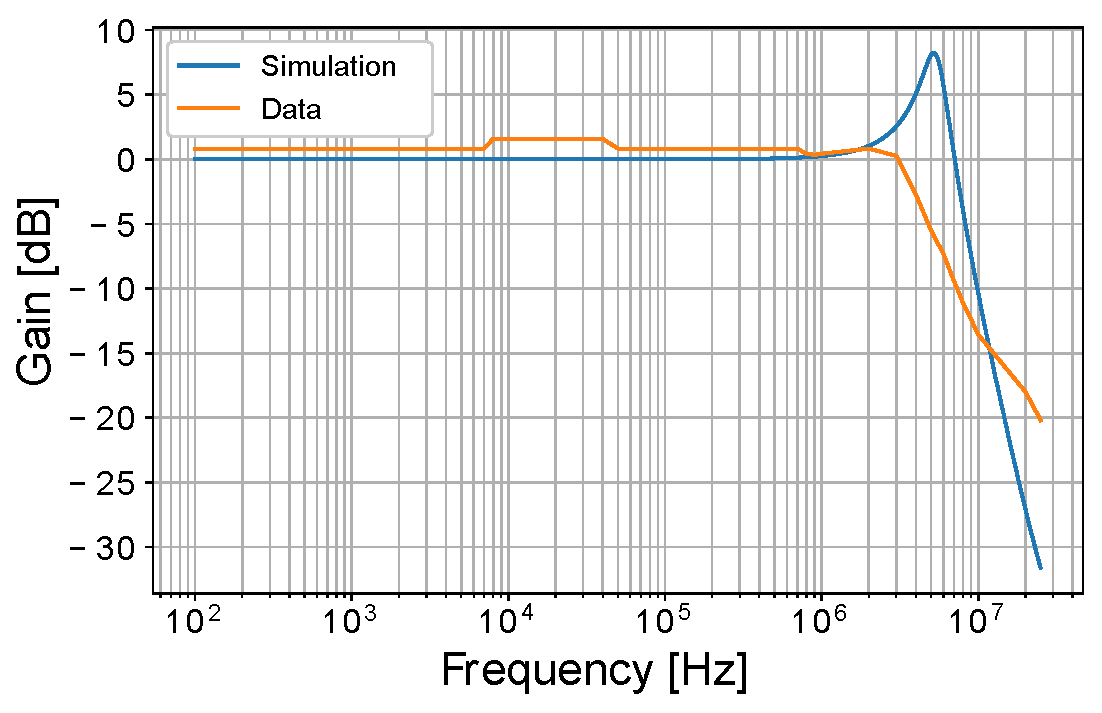
\includegraphics[width=0.6\textwidth]{Figures/Integrador_Bode.eps}
\caption{Simulated (blue) and measured (orange) Bode diagram of the integrator. The circuit frequency cut was $\sim$4\,MHz (-3\,dB) preserving the input signal amplitude (unitary gain) under $\sim$3\,MHz.}
\label{fig::bode}
\end{center}
\end{figure}

\subsection{Noise analysis}

We characterized the circuit noise by analyzing its output without input signal. The noise presents a normal distribution centered in 0\,mV and with a standard deviation $\sim$ 3.49\,mV as shown in Fig. \ref{fig::intnoise}.


\begin{figure}[h!]
\begin{center}
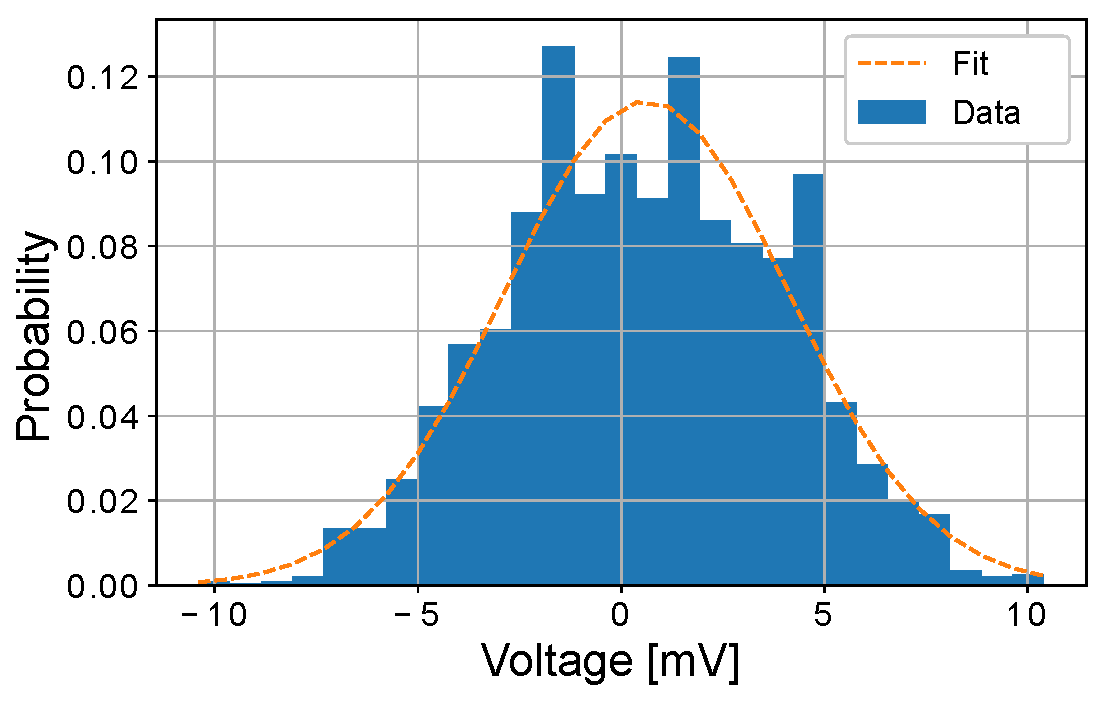
\includegraphics[width=0.6\textwidth]{Figures/Ruido_Ana.eps}
\caption{Front-end electronics noise distribution. The circuit output varies around the base line with a standard deviation of 3.49\,mV.}
\label{fig::intnoise}
\end{center}
\end{figure}

\subsubsection{Signal spectral analysis}

\begin{figure}[h!]
\begin{center}
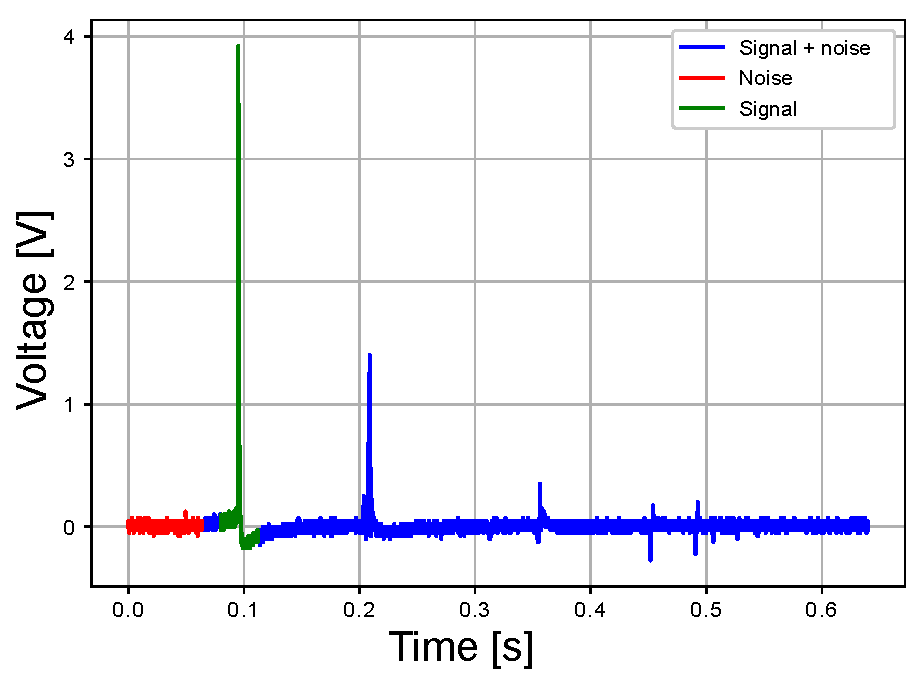
\includegraphics[width=0.6\textwidth]{Figures/Descarga.eps}
\caption{Lightning signal recorded on March 2, 2020, at Bucaramanga-Colombia. The signal was split into noise (red-line) and discharge (green-line) portions to analyze their frequency spectrum.}
\label{fig::descarga}
\end{center}
\end{figure}


We analyzed the lightning signal frequency spectrum to establish the sampling frequency of the digitization stage. The signal was recorded by an oscilloscope TEKTRONIX TDS 2002B (1 GS/s). Fig. \ref{fig::descarga} shows the 02032020 (March 2, 2020) lightning event recorded at Bucaramanga, Colombia. 

The signal presents a first return stroke of $\sim$4\,V (200\,V/m above the antenna place) with subsequent strokes at $\Delta t \sim$0.1\,s, $\sim$0.25\,s, $\sim$0.35\,s, and $\sim$0.39\,s. The recording window was set to 0.7\,s. 

We characterized the noise (red) and signal (green) spectrum by applying the FFT in two portions of the recorded signal. The principal frequency components of the lightning signal are below $\sim$4\,kHz, while noise components extend to $\sim$20\,kHz.

\begin{figure}[h!]
\begin{center}
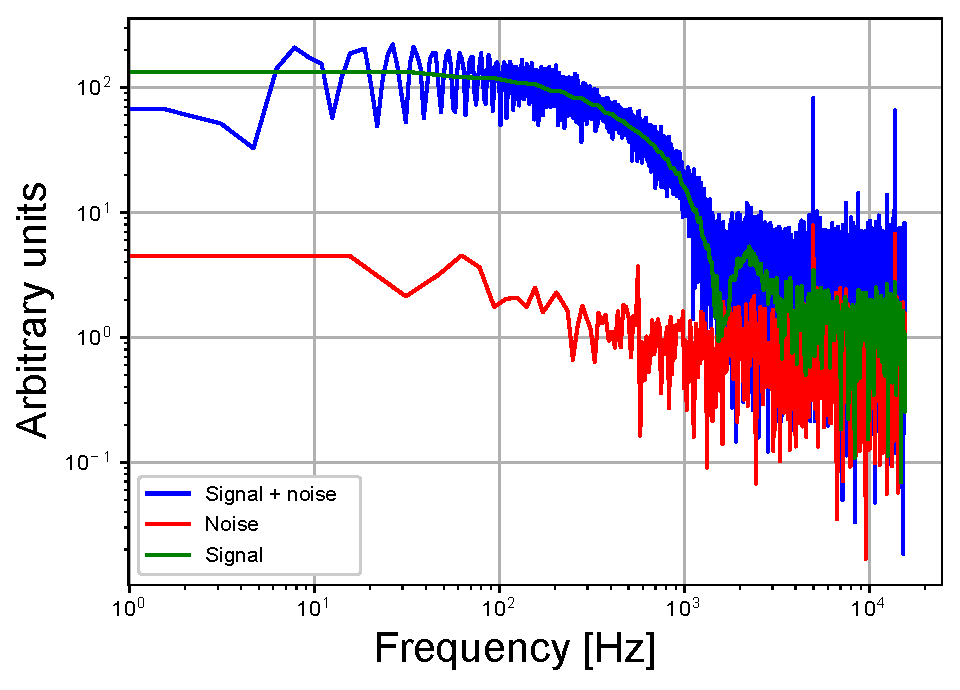
\includegraphics[width=0.6\textwidth]{Figures/Evento_FFT.eps}
\caption{Fast Fourier Transform of the recorded signal. The frequency components of the discharge (green-line) are below $\sim$4\,kHz and the noise (red-line) extend to $\sim$20\,kHz.}
\label{fig::fftsignal}
\end{center}
\end{figure}

\subsection{Digitization and storage}

A 12-bit ADC (AD9235\footnote{\url{https://www.analog.com/en/products/ad9235.html}}) digitizes the lightning signal with a sampling frequency of 100\,kHz. The ADC input range was set to 2\,V where an ADC unit represents $\sim$488.2\,$\mu$V. 

A Spartan 6 FPGA Development Board (Mimas) manages the acquisition process. The FPGA generates the 1\,MHz ADC clock, applies the voltage-over-threshold trigger, addresses the signal data to a 16-Mbit flash memory (SST39VF1602C\footnote{\url{https://www.microchip.com/wwwproducts/en/SST39VF1602C}}), and transmits the data to the Raspberry Pi.

When the lightning event exceeds the detection threshold ($\sim$ 500\,mV) the data acquisition system records a 1.2\,s window at 100\,kHz. Each recorded event has an associated time stamp with 10\,ns resolution and GPS synchronization (UTC).

The lightning detection hardware was tested by injecting square pulses (50\,ms width and 1\,V height) emulating electrical discharges from a Tektronix AFG1022 signal generator. Fig. shows the test results. The fine time stamp was synchronized with the GPS PPS signal (yellow-line). The emulated lightning signal occurred at $\sim$499\,ms from the last PPS. The measured occurrence time is represented by the red dashed-line.

\begin{figure}[h!]
\begin{center}
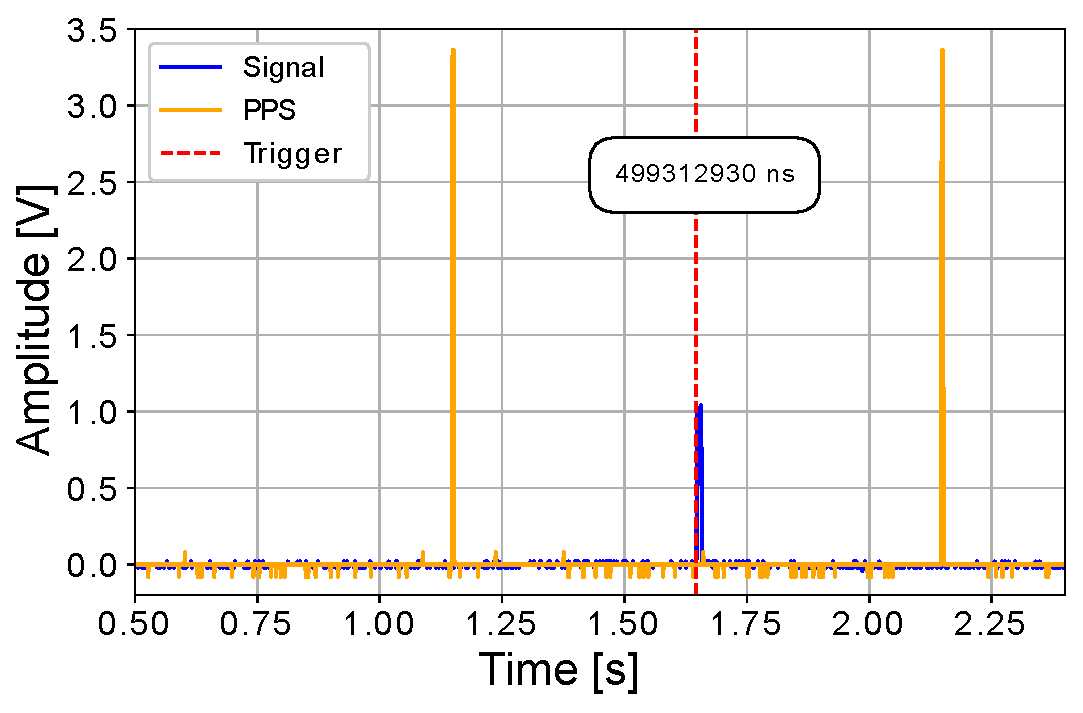
\includegraphics[width=0.6\textwidth]{Figures/test.eps}
\caption{The lightning detection system was stimulated by a square pulse (50\,ms width and 1\,V height) (blue-line) from a Tektronix AFG1022 signal generator. The fine time stamp (red dashed-line) is relative to the PPS signal (yellow-line). The occurrence time of the emulated lightning signal was measured $\sim$499\,ms. }
\label{fig::fftsignal}
\end{center}
\end{figure}

\subsection{Monitoring station}

The monitoring station includes the lightning detection system, the atmospheric electric field mill, and environmental sensors. A single computer board (Raspberry Pi) operates the station running under Raspbian Wheezy. The BME280\footnote{\url{https://www.bosch-sensortec.com/products/environmental-sensors/humidity-sensors-bme280/}} sensor measures temperature, relative humidity, and atmospheric pressure with an accuracy of $\pm$1 $^{\circ}$C, $\pm$3 $\%$RH, and $\pm$1 hPa respectively. 

A Venus 638FLPx chip performs the monitoring station global positioning with a spatial accuracy of 2.5 m and a time accuracy of 60 ns. The GPS transmits the data via UART protocol at 9600 bauds and needs a 3.3\,V powering. The positioning data contains UTC, latitude, N/S indicator, longitude, E/W indicator, and altitude. The time synchronization of the acquisition system depends on the PPS signal. The localization of the lightning strike point is estimated by using a trilateration algorithm based on the GPS data \cite{MialdeaFlor2019}. A picture of the station hardware is displayed in Fig. \ref{fig::station}.

%The monitoring station data can be acceded by an Ethernet link from a central server.

\begin{figure}[h!]
\begin{center}
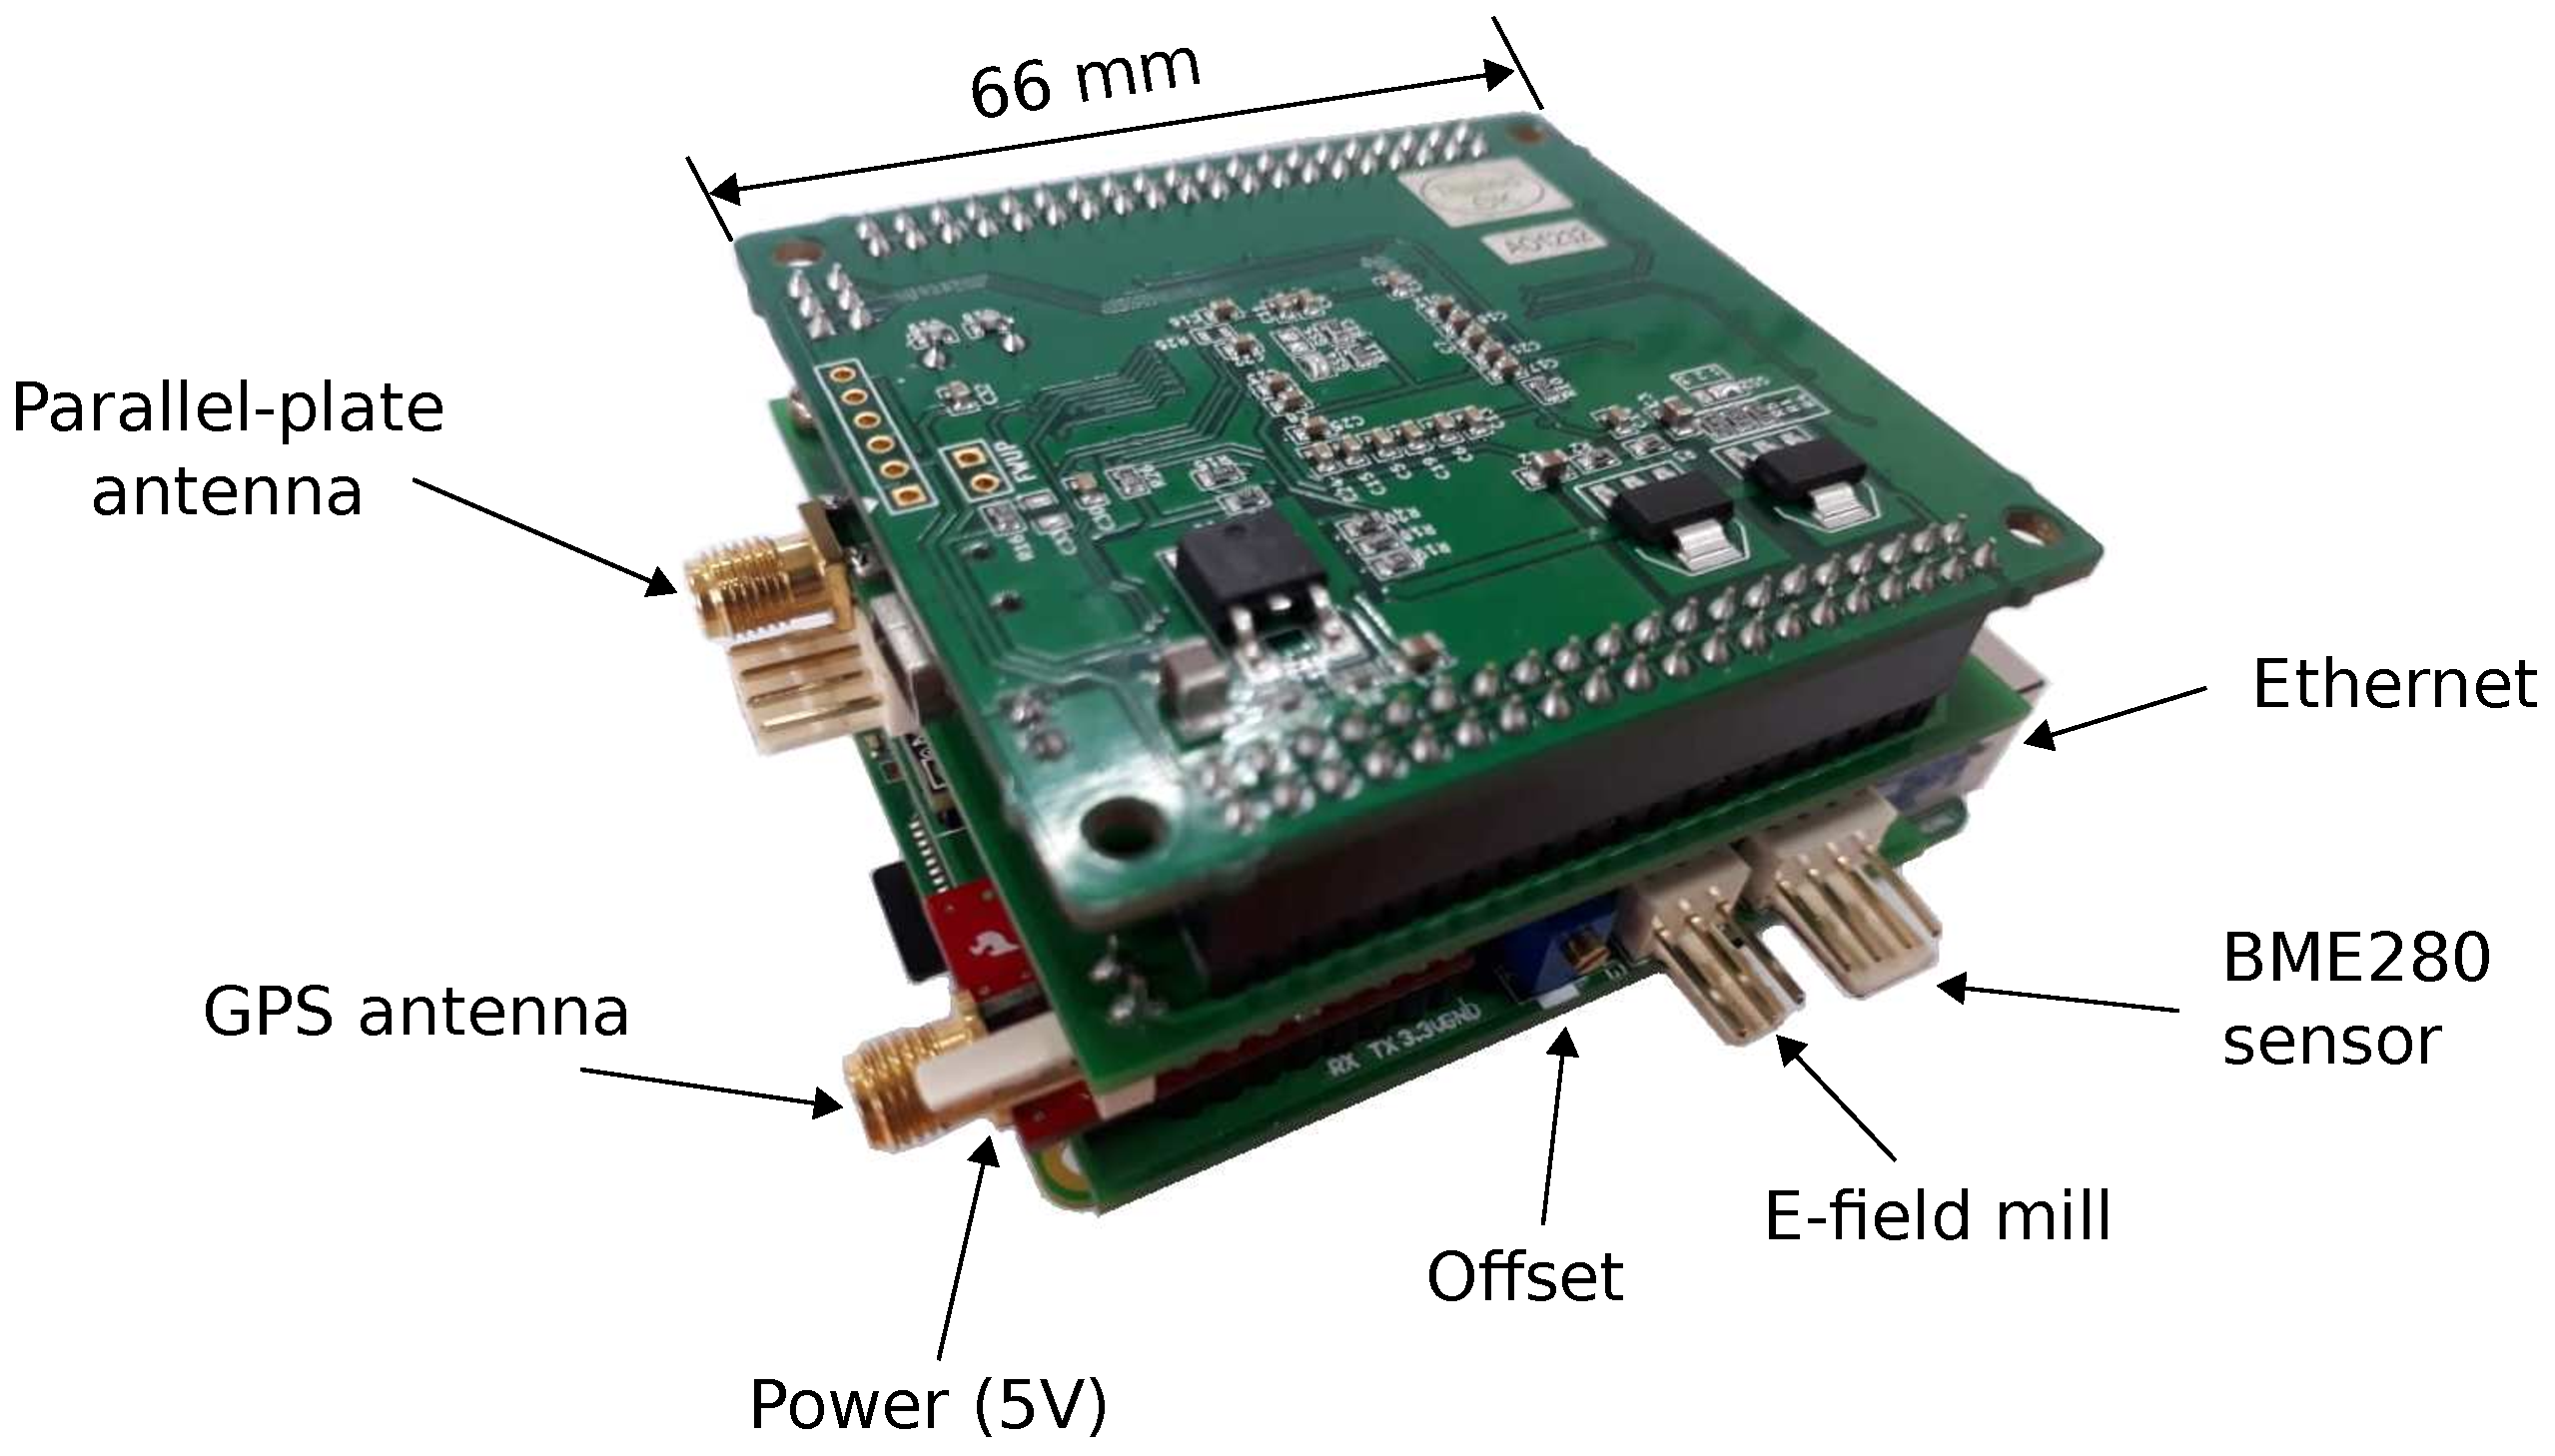
\includegraphics[width=0.7\textwidth]{Figures/Station.eps}
\caption{Monitoring station hardware.  The lightning and environmental readout electronics stack on the Raspberry Pi single computer board as removable shields. External connectors for powering, weather sensors, GPS antenna, parallel plate antenna, E-field mill, and Ethernet encircle the station hardware.}
\label{fig::station}
\end{center}
\end{figure}

The hardware is arranged in 4 layers, from the bottom to the top, the Raspberry Pi 2, the environmental layer (PSOC 5LP, GPS Venus 638FLPx, and BME280), the Spartan 6 FPGA Development Board, and the lightning detection system.

\subsection{Mechanical structure}
A waterproof plastic enclosure (IP65 standard) contains the station hardware. The box has a transparent cover to monitor the station status LEDs. Four plastic screws attach the enclosure cover with the body separated by a rubber seal.

Two case external SMA connectors input the GPS and parallel plate antenna signals. A 4-pin XLR connects the electric field mill (signal, phase, and GND). A second 4-pin XLR connector inputs the environmental sensor BME280 (SDA, SCL, 3.3\,V, and GND), and a 7-pin XLR connector powers the station (5\,V and GND). All the connectors are on the bottom side of the plastic enclosure.

\begin{figure}[h!]
\begin{center}
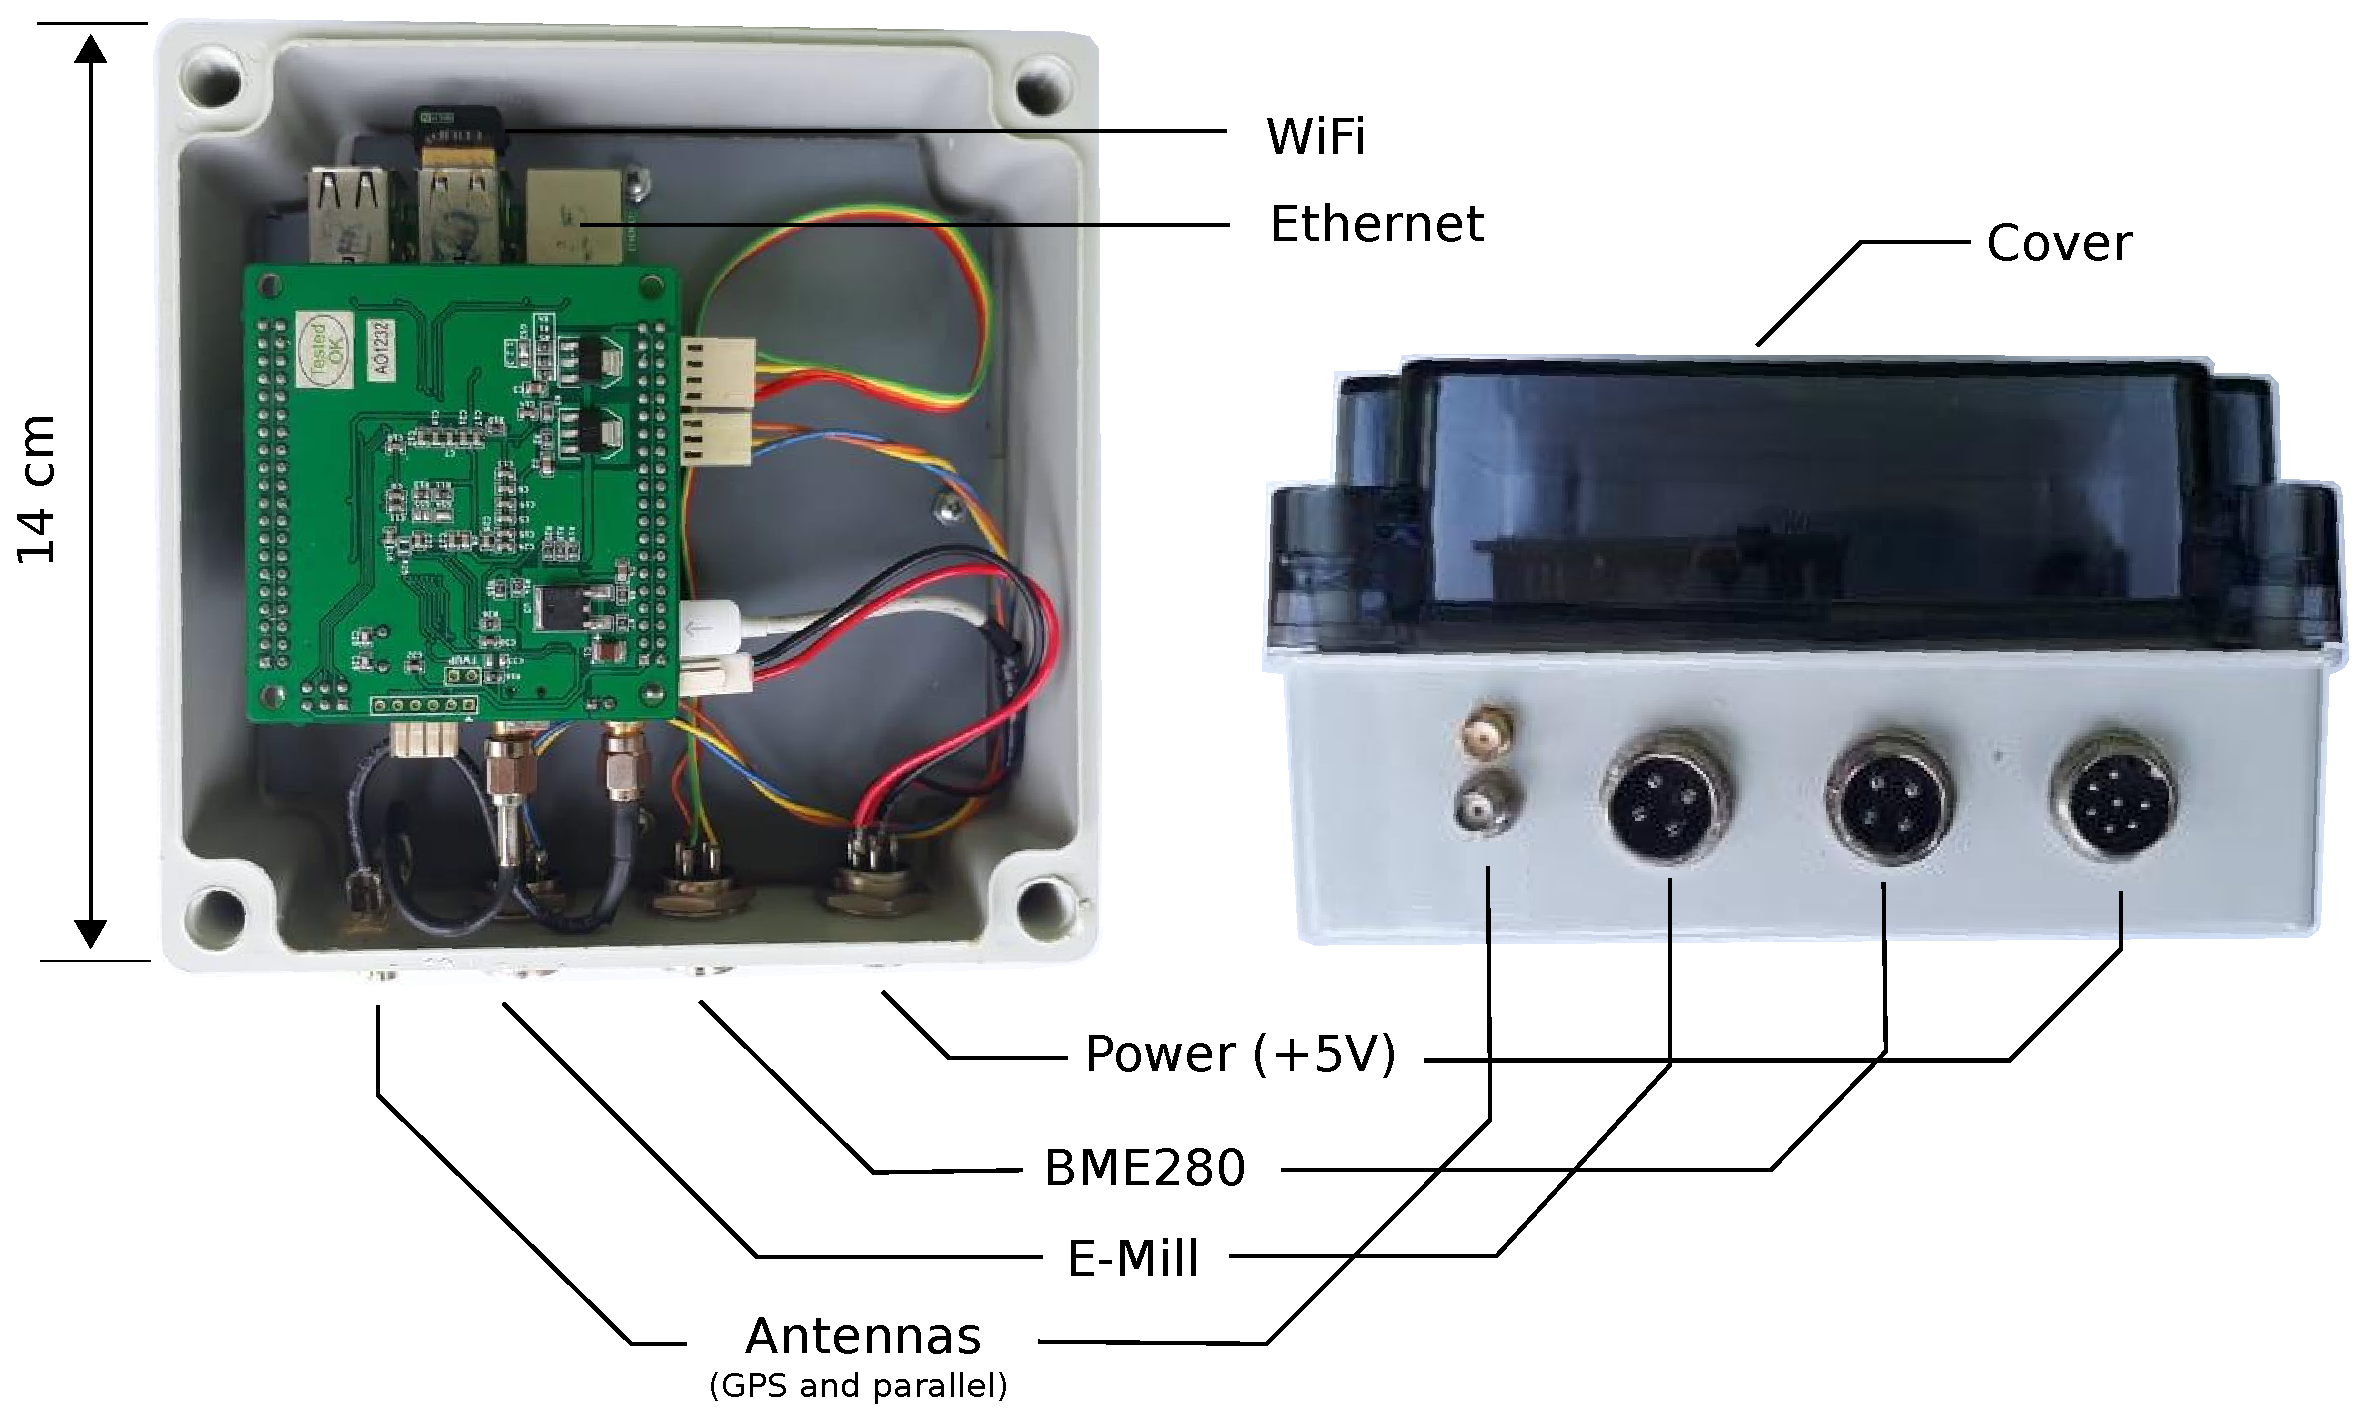
\includegraphics[width=0.9\textwidth]{Figures/Station_structure.eps}
\caption{Monitoring station enclosure. Two SMA connectors input the parallel plate and GPS antenna signals. The E-field mill, BME280, and power supply are connected using XLR plugs.}
\label{fig::station}
\end{center}
\end{figure}

\subsection{Data files}

The monitoring station runs concurrently two acquisition python codes. The first records the atmospheric electric field and environmental data and the second stores the lightning data.

The environmental acquisition code hourly creates a data file named \textbf{Datos\_YYYY\_MM} \textbf{\_DD\_HH.dat} (YYYY-year, MM-month, DD-day, and HH-hour), taking into account the UTC data from the GPS. The environmental data file starts with the station metadata (Station name, code version, and geographical location) labeled with \textbf{#} character. Sensors data contain UTC, atmospheric electric field, temperature, pressure, and humidity. The PPS signal stars every new data row acquisition.

The lightning detection code starts the acquisition when an interruption signal from the FPGA trigger system detects a new event. This methodology avoids memory wastage typical of continuous recording at high sampling frequencies. A file named \textbf{Lighting\_YYYY\_MM} \textbf{\_DD\_HH\_mm.dat} (mm-minute) stores the lightning waveform (120000 samples - 1.2\,s) and the nano-second time stamp. The file metadata contains the code version, station geo-position (latitude and longitude), vertical resolution (2.048\,mV/UADC), sampling period (10\,$\mu$s), and event time (seconds).

\subsection{First measurements}

In this section, we show preliminary measurements recorded during a thunderstorm event on 2019-11-09 at Bucaramanga-Colombia. The event lasts about 2 hours, recording a maximum electric field peak of $\sim$-15\,kV/m. The atmospheric electric field recovers the steady-state after at least half-hour of continuous lightning activity, showing a ripple $\sim$4\,kV/m. 

The thunderstorm cloud-base height ($\sim$2\,km) was estimated by using a model based on the relative humidity and temperature \cite{Lawrence2005}. The cloud-to-ground potential is proportional to the measured electric field and inverse to the cloud base distance. The atmospheric potential was $\sim$27\,MV at the electric field maximum.

Fig. \ref{fig::event} shows the environmental temperature dropped 3.5$^{\circ}$ during the thunderstorm beginning. The relative humidity decreased from 88$\%$ to 76$\%$ due to a wind speed increment (dissipation of the water molecules). 

\begin{figure}[h!]
\begin{center}
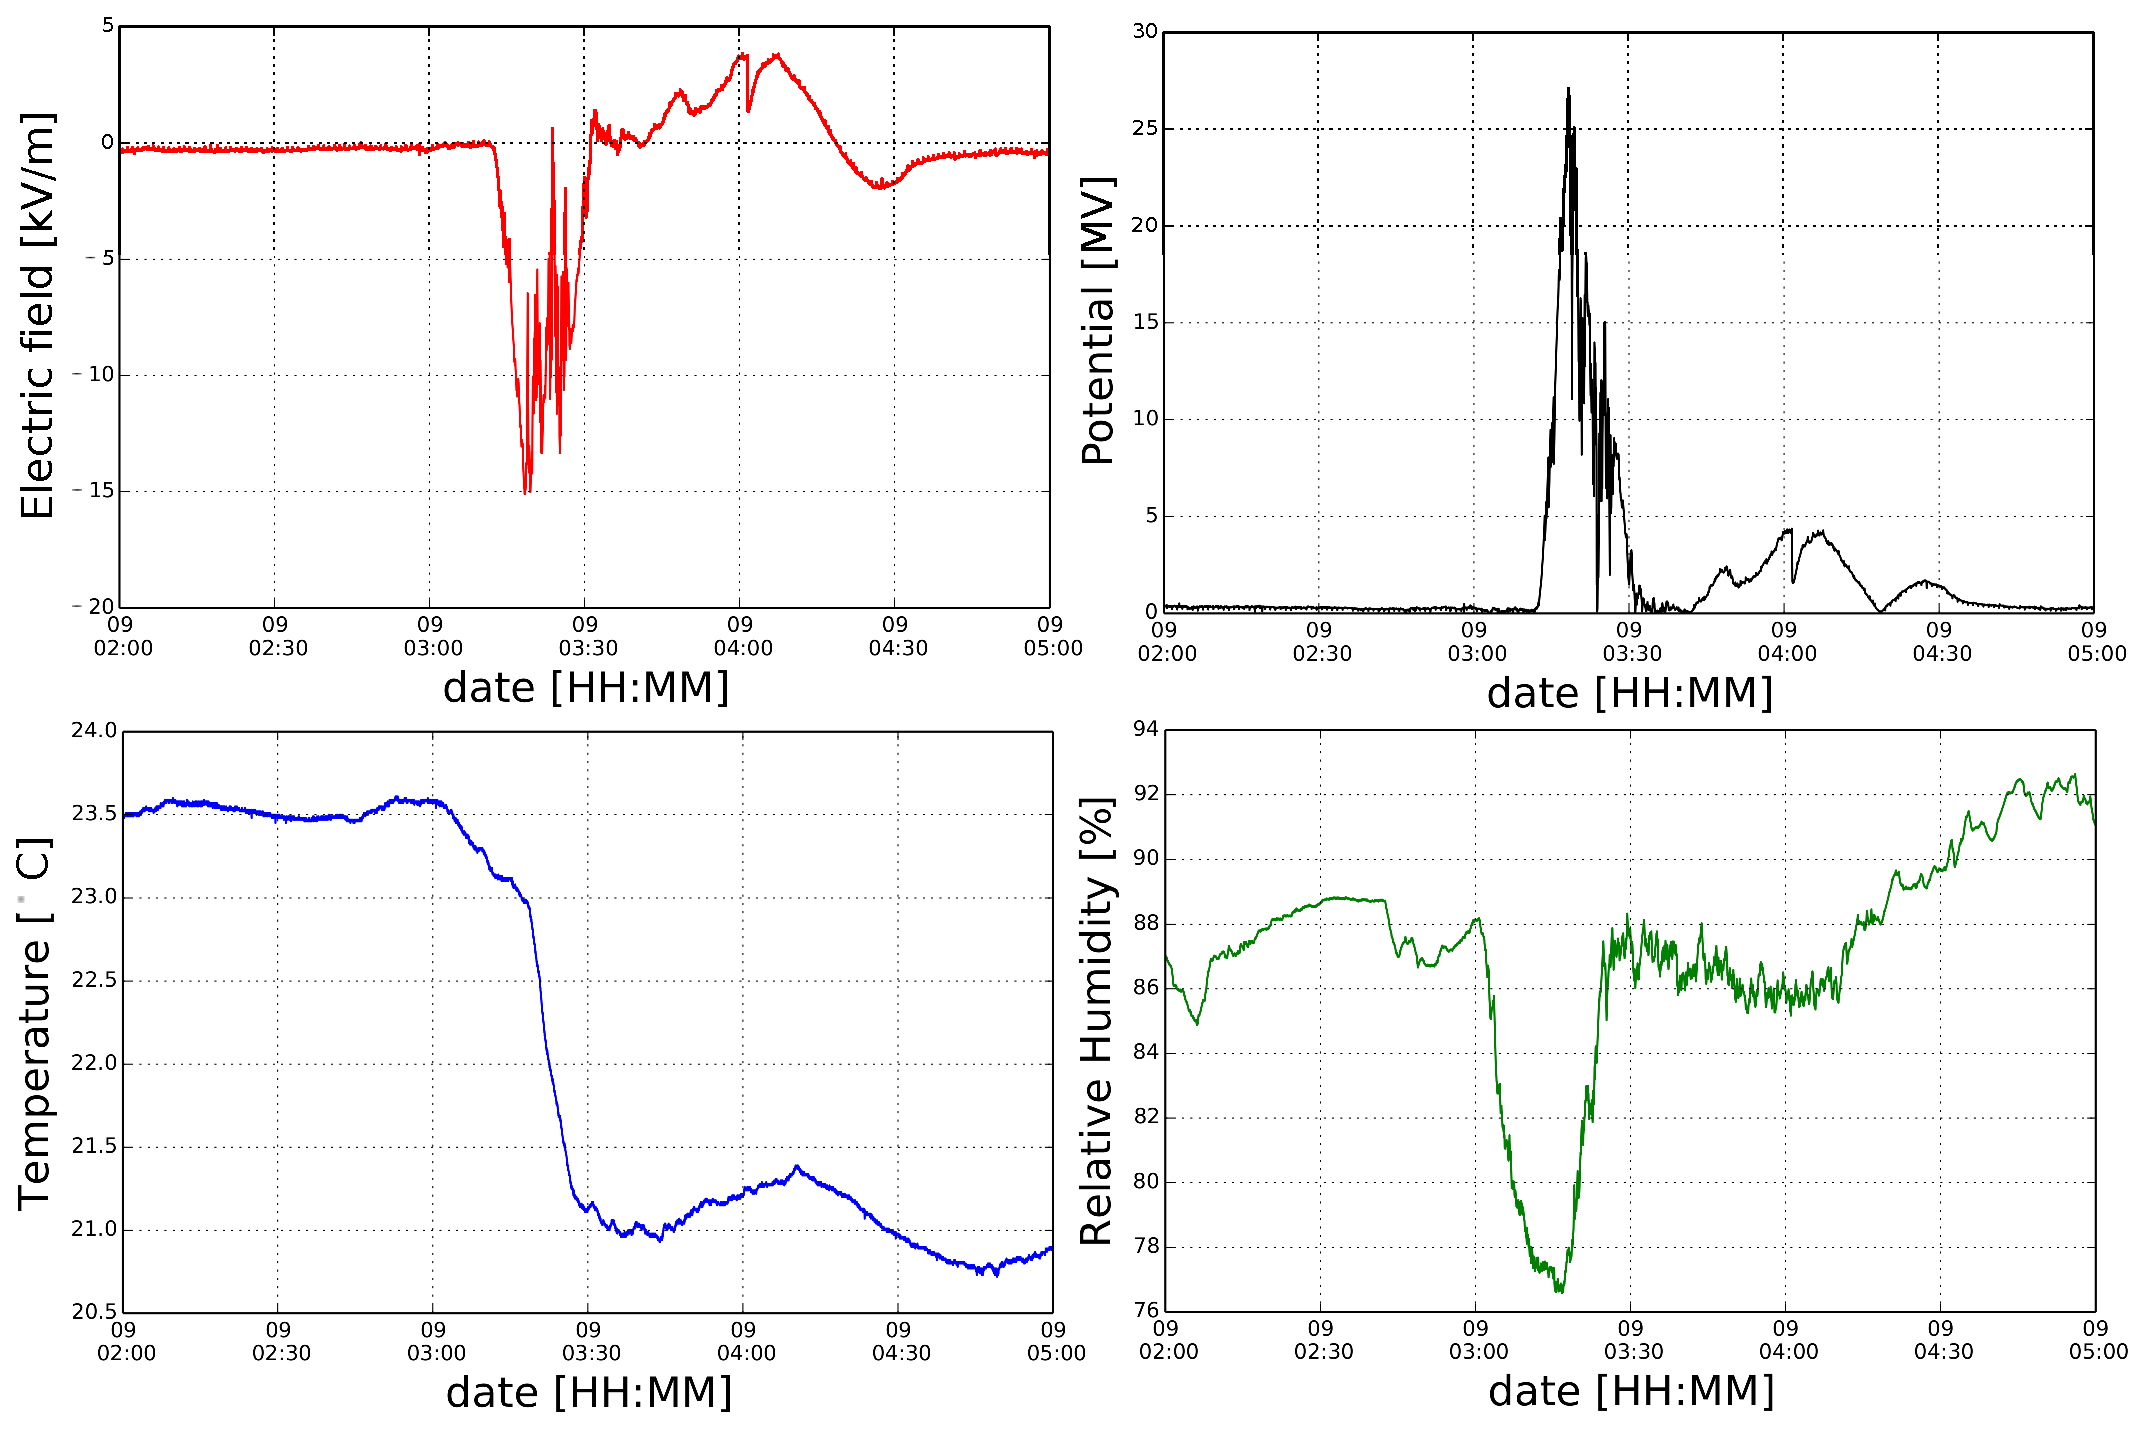
\includegraphics[width=1\textwidth]{Figures/Event.eps}
\caption{Results of the atmospheric data taking during the 2019-11-09 thunderstorm episode. A negative electric field (red-line) with a maximum of -15\,kV/m was recorded after the thundercloud formation $\sim$ 2 km above the observation place. The absolute value of the cloud-ground potential (black-line) was estimated using the atmospheric electric field and the cloud base. The cloud base was modeled by using measurements of temperature (blue-line) and relative humidity (green-line).}
\label{fig::event}
\end{center}
\end{figure}

At least four lightning events occurred during the thunderstorm period. Such discharges released an electric field $>$5\,kV/m as shown in Fig. \ref{fig::light}. The first event represented an electric field variation of close 8.5 kV/m in less than one minute. The thundercloud charge accumulation was released during ($\sim$ 10 min) by lightning discharges until the electric field decreased around the baseline. The cloud-to-ground current estimation shall be possible if we know the lightning strike distance.

\begin{figure}[h]
\begin{center}
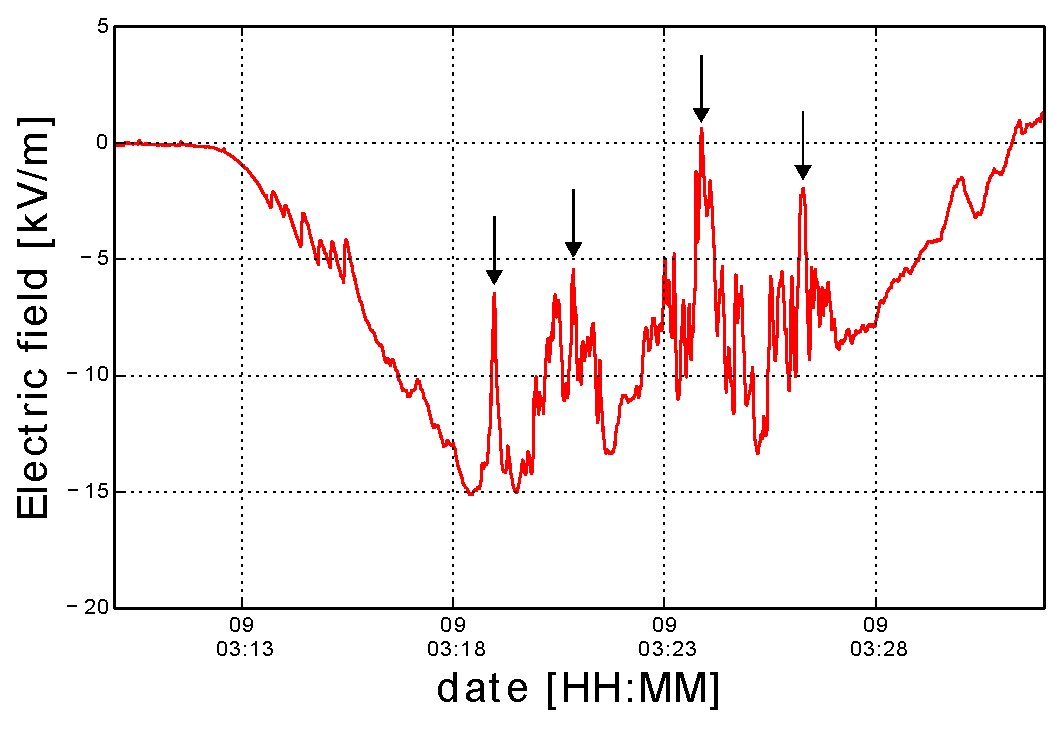
\includegraphics[width=0.6\textwidth]{Figures/lightning.eps}
\caption{Lightning events (black-arrows) recorded by the monitoring station during the 2019-11-09 thunderstorm. }
\label{fig::light}
\end{center}
\end{figure}
 

\section{Conclusions}

A direct relationship between the atmospheric electric field and the flux of charged particles at ground level have been demonstrated by several studies. In this note, we presented a monitoring station design and first measurements of the atmospheric electric field, lightning, and environmental variables (temperature and relative humidity) involved in thunderstorm episodes. The station acquisition system fulfills timing and triggering requirements needed to cross the recorded data with the counting rate measurements of particle detectors.

Preliminary measurements showed a correlation between the environmental temperature and relative humidity during the 2019-11-09 thunderstorm development. The atmospheric electric field rose to -15\,kV/m with a cloud-ground potential $\sim$27\,MV. Additionally, we identified some lightning events which caused an electric field variation of the order of 8.5\,kV/m.


\section{Future Work}
We are planning the design and implementation of a photovoltaic system to supply the monitoring station in remote environments. 


\bibliographystyle{unsrt}
\bibliography{biblio.bib}

% \newpage
% \appendix
% \section{Potential and cloud-base estimation}
\label{app::cloudbase}

El campo eléctrico lento es producido por la acumulación de carga en las nubes; el conjunto atmósfera-tierra se puede considerar como un capacitor de placas paralelas. La expresión de la Eq. \ref{potencial} describe el comportamiento del potencial que se genera entre las nubes y la tierra, con $E$ como el campo eléctrico y $d$ la altura de la base de la nube.
\begin{equation}
    V = Ed
    \label{potencial}
\end{equation}
G. Lawrence et. al. en su trabajo \textbf{"The Relationship between Relative Humidity and the Dewpoint Temperature in Moist Air"} \cite{lawrence2005relationship} propone una expresión para la aproximación la altura de la base de la nube cúmulo ($Z_{lcl}$) y su relación con la temperatura de rocío ($t_{d}$) y la temperatura del aire ($t$) a nivel de suelo tal como se observa en la Eq. \ref{alt}.
\begin{equation}
    d\approx 125\left (t - t_{d}\right )
    \label{alt}
\end{equation}
La temperatura a la que se condensa el vapor de agua en una muestra de gas se le llama temperatura de punto de rocío y su valor depende de la humedad relativa del gas ($RH$) \cite{lawrence2005relationship}, tal como se observa en la Eq. \ref{td}.
\begin{equation}
    td \approx t - \left ( \frac{100 - RH}{5}\right)
    \label{td}
\end{equation}

\end{document}
